\section{Aseguramiento de la Calidad}\label{sec:aseguramientoDeLaCalidad}

Para cumplir con los objetivos establecidos, se desarrolló un conjunto de prácticas que aseguran la calidad tanto en la 
gestión del proceso como en el producto final. Estas prácticas fueron adoptadas por todo el equipo y se aplicaron 
consistentemente a lo largo de todas las fases del proyecto.

\subsection{Aplicación de estándares}
Desde el inicio, se definieron estándares claros tanto para los procesos como para el producto final. Algunos de estos 
estándares fueron definidos internamente por el equipo, mientras que otros se basaron en recomendaciones de la industria.

\subsection{Estándares de codificación}
Se implementaron principios de Clean Code para garantizar una estructura y sintaxis claras en el código fuente, facilitando 
la comprensión y modificabilidad del software. El código se escribió en inglés para mejorar su legibilidad y facilitar la 
expansión futura del equipo de desarrollo. Se aplicaron los principios SOLID para asegurar que el código sea modular, fácil 
de mantener y modificado, maximizando su efectividad y reduciendo costos de mantenimiento.
En la tabla siguiente se detallan los diferentes estándares aplicados al código fuente en este proyecto.

\begin{table}[H]
    \centering
    \begin{tabular}{p{3cm} p{10cm}}
    \hline
    \rowcolor[HTML]{C0C0C0} 
    \textbf{Estándar} & \textbf{Descripción}                                                                                     \\ \hline
    \textbf{Clean Code} & Se aplicaron principios de Clean Code para garantizar una estructura y sintaxis claras en el código fuente. \\ \hline
    \textbf{SOLID}     & Se aplicaron los principios SOLID para asegurar que el código sea modular, fácil de mantener y modificar.       \\ \hline
    \textbf{Inglés}    & El código se escribió en inglés para mejorar su legibilidad y facilitar la expansión futura del equipo de desarrollo. \\ \hline
    \end{tabular}
    \caption{Estándares de codificación}
    \label{tab:estandaresCodificacion}
\end{table}

\subsection{Estándares de documentación}

Para los documentos generados durante el proyecto, se siguieron las directrices de la Universidad ORT Uruguay, 
complementadas con lineamientos específicos del equipo para garantizar coherencia y uniformidad.
En la tabla \ref{tab:estandaresDocumentacion} se detallan los diferentes estándares aplicados a la documentación en este proyecto.


\begin{table}[H]
    \centering
    \begin{tabular}{p{3cm} p{10cm}}
    \hline
    \rowcolor[HTML]{C0C0C0} 
    \textbf{Estándar} & \textbf{Descripción}                                                                                     \\ \hline
    \textbf{Normas de la Universidad ORT} & Se siguieron las directrices de la Universidad ORT Uruguay para la redacción de documentos. \\ \hline
    \textbf{Uniformidad}     & Se establecieron lineamientos específicos del equipo para garantizar coherencia y uniformidad en la documentación.       \\ \hline
    \end{tabular}
    \caption{Estándares de documentación}
    \label{tab:estandaresDocumentacion}
\end{table}

\subsection{Plan de Pruebas}
\subsubsubsection{Objetivo}

Evaluar las funcionalidades del producto de software para verificar y validar que satisface las necesidades y expectativas del cliente. El plan 
busca garantizar la calidad mediante pruebas que cubren tanto aspectos funcionales como no funcionales, con un enfoque ágil e iterativo.

\subsubsubsection{Alcance}
El plan de pruebas cubre la verificación de las funcionalidades del sistema, su compatibilidad con el ambiente de uso y la evaluación de la 
experiencia de usuario bajo condiciones realistas. Además, se incluyen pruebas de rendimiento bajo alta demanda. No se realizarán pruebas 
específicas de seguridad debido a que se asume que el sistema será utilizado en un entorno controlado y seguro.

\subsubsubsection{Equipo}
Se asginan los roles y tareas a cada integrante descritos en la tabla \ref{tab:rolesPruebas}.

\begin{table}[H]
    \centering
    \begin{tabular}{p{3cm} p{3cm} p{8cm}}
    \hline
    \rowcolor[HTML]{C0C0C0} 
    \textbf{Nombre} & \textbf{Rol} & \textbf{Responsabilidad}                                                                                     \\ \hline
    Horacio Ábalos & QA y Tester & Planificación y ejecución de pruebas funcionales y no funcionales. Cobertura de requisitos. Gestión de herramientas de automatización. Identificación y seguimiento de defectos. Colaboración en la resolución de problemas. Pruebas exploratorias. \\ \hline
    Cristian Palma & PO y Tester & Definición de la visión del producto. Priorización de backlog. Alineación de requisitos. Revisión y aceptación de entregas. Retroalimentación continua. Identificación y seguimiento de defectos. Pruebas funcionales y exploratorias. \\ \hline
    Federico Alonso & Arquitecto y Revisor de Código & Diseño y validación de la arquitectura. Decisiones sobre tecnología. Definición de componentes y su interacción. Resolución de problemas técnicos. Revisión de código y decisiones de diseño. \\ \hline
    Ramiro Gallego & Tester y Revisor de Código & Pruebas funcionales y exploratorias. Revisión y mejora de calidad de código. Identificación de defectos. Validación de la implementación y documentación de pruebas. \\ \hline
    \end{tabular}
    \caption{Roles en el equipo de pruebas}
    \label{tab:rolesPruebas}
\end{table}


\subsubsubsection{Estrategia}

\subsubsubsubsection{Risk-Based Testing}
Se implementará una matriz de riesgo para priorizar las pruebas en base a dos factores:

\begin{itemize}
    \item \textbf{Probabilidad de fallo:} complejidad de la solución, dependencia de sistemas externos.
    \item \textbf{Impacto en el negocio:} funcionalidades críticas como la gestión de incidentes, cálculo y 
    obtención de datos de barcos y meteorológicos.
\end{itemize}

% insertar una imagen
\begin{figure}[H]
    \centering
    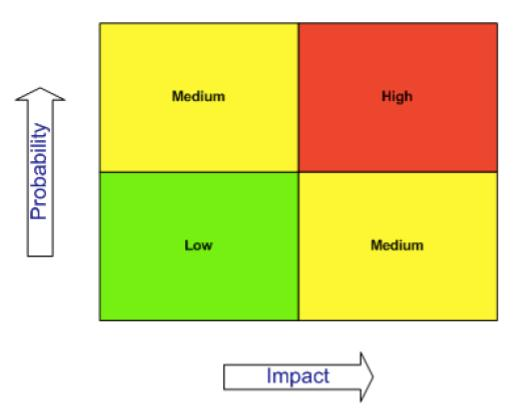
\includegraphics[width=0.8\textwidth]{../imagenes/secciones/8-Gestion-de-la-Calidad/matriz de testing basado en riesgo.jpg}
    \caption{Matriz de testing basado en riesgo}
    \label{fig:matriTestRiesgo}
\end{figure}

Esta matriz ayudará a centrar los esfuerzos de prueba en las áreas del sistema con mayor riesgo y probabilidad de impacto. 
De ella se desprende que:

\begin{itemize}
    \item Alta probabilidad y alto impacto (rojo): Debe probarse primero.
    \item Alta probabilidad y bajo impacto (amarillo): Se debe probar si hay tiempo disponible.
    \item Baja probabilidad y alto impacto (amarillo): Debe probarse si se dispone de tiempo suficiente.
    \item Baja probabilidad y bajo impacto: Se puede posponer para futuras iteraciones.
\end{itemize}

\begin{figure}[H]
    \centering
    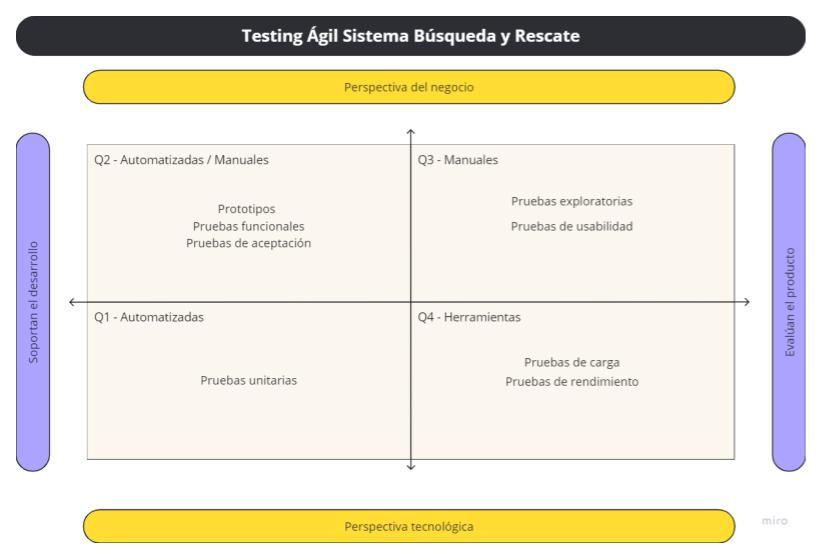
\includegraphics[width=0.8\textwidth]{../imagenes/secciones/8-Gestion-de-la-Calidad/Cuadrantes testing agil .jpg}
    \caption{Cuadrantes de testing ágil}
    \label{fig:cuadrantesTesting}
\end{figure}


\subsubsubsubsubsection{Q1 - Pruebas unitarias}
Estas pruebas serán realizadas sobre la lógica de la funcionalidad clave, el Cálculo del Área de Búsqueda, utilizando 
el framework Jest. El objetivo es asegurar que cada unidad de código funcione correctamente y de manera aislada. 
Las pruebas se ejecutarán automáticamente en cada merge a la rama develop, verificando así la estabilidad continua del sistema. 
Además, se incluirán pruebas en otras áreas de la lógica que estén acopladas a estas funcionalidades críticas para evitar regresiones.

\subsubsubsubsubsection{Q2 -  Pruebas Funcionales y de Aceptación}
\subsubsubsubsubsubsection{Pruebas funcionales}
En estas pruebas se consideran aspectos relevantes como las integraciones del sistema con servicios externos para la obtención de datos 
climáticos y la información de barcos cercanos a un incidente. Estas pruebas serán automatizadas para ejecutarse continuamente durante 
regresiones y en el pipeline de CI/CD. Se emplearán herramientas como Jest y los resultados se verificarán automáticamente en cada merge 
a la rama develop.

\subsubsubsubsubsubsection{Pruebas de aceptación}
Estas pruebas serán automatizadas utilizando Cucumber y se basarán en escenarios escritos en el formato Como [rol] quiero [funcionalidad] 
para [beneficio]. El objetivo del equipo es integrar estas pruebas en el pipeline solamente para las funcionalidades clave, permitiendo 
una rápida verificación del estado del sistema con cada merge a develop. Estas pruebas se enfocan en validar que el sistema cumple con los 
criterios de aceptación definidos por el Product Owner y las necesidades del usuario final.

\subsubsubsubsubsection{Q3 - Pruebas Exploratorias y de Usabilidad}
\subsubsubsubsubsubsection{Pruebas exploratorias}
Serán realizadas también pruebas exploratorias por diferentes integrantes del equipo. Estas pruebas deben ser ejecutadas por un integrante 
diferente al que haya desarrollado la funcionalidad.
Se utilizará la siguiente plantilla para estas sesiones exploratorias.

[link a la plantilla: https://docs.google.com/document/d/1nvdvL7GpPiP9tGPadTUYDdJpAkJrE9nZXniJSIlVs88/edit]

\subsubsubsubsubsubsection{Pruebas de usabilidad}
Considerando el contexto específico del sistema, y que será utilizado por usuarios altamente capacitados, el centro del esfuerzo no estará 
en realizar pruebas de usabilidad. Independientemente de lo anterior, realizaremos encuestas a los usuarios luego de la gestión de un incidente 
que nos proporcione la retroalimentación para verificar si el sistema es fácilmente utilizable y permite completar tareas mejorando los tiempos 
empleados actualmente.\\
En tal sentido se liberará la primera versión del sistema para validar las funcionalidades en entornos controlados y con usuarios reales. Durante 
esta primera versión se recolectará feedback utilizando encuestas post-gestión de incidente.\\
Las encuestas serán cortas y específicas, asegurándonos de recolectar retroalimentación sin interrumpir las tareas. Se implementará un sistema de 
retroalimentación multivaluado que nos permita entender si:

\begin{itemize}
    \item ¿El usuario considera necesario modificar el sistema?
    \item ¿El sistema cumple tus expectativas en cuanto a facilidad de uso?
    \item ¿Cómo es calificada la experiencia general utilizando el sistema?
    \item ¿El tiempo empleado en realizar los cálculos acorta significativamente el tiempo de las tareas?
\end{itemize}

En la siguiente plantilla se propone la encuesta inicial a ser incluida en un formulario que será visualizado luego de cerrar un incidente.

[link a la plantilla: https://docs.google.com/document/d/1uuIf-cvXXNpDl3GCFkLb5_kfsGJymRFhI9w9hSoFSag/edit]

\subsubsubsubsubsection{Q4 - Pruebas de Performance}

Las pruebas de rendimiento se realizarán utilizando K6, una herramienta especializada para simular condiciones de alta carga y estrés. El objetivo 
es evaluar cómo el sistema maneja situaciones críticas, midiendo el tiempo de respuesta, la capacidad de procesar múltiples solicitudes simultáneas y 
la estabilidad bajo picos de uso. Estas pruebas se integrarán en el pipeline de CI/CD, permitiendo detectar problemas de rendimiento en etapas tempranas 
del desarrollo. El uso de K6 permitirá automatizar las simulaciones y obtener métricas detalladas para ajustar y optimizar el rendimiento de la aplicación.

[TODO: Ajustar según los RNF finales]

\subsubsubsubsection{Criterios de Ejecución y Finalización}

\begin{itemize}
    \item Inicio: Las pruebas comenzarán una vez superadas todas las pruebas unitarias.
    \item Finalización: Las pruebas finalizarán cuando:
    \begin{itemize}
        \item Todos los casos de prueba de prioridad alta (1) se ejecuten sin fallos.
        \item Al menos el 60\% de los casos de prueba de prioridad media (2) se ejecuten sin fallos.
    \end{itemize}
\end{itemize}

La tabla \ref{prioridadCasosPrueba} establece la prioridad para la ejecución de los casos de prueba:

\begin{table}[H]
    \centering
    \begin{tabular}{p{3cm} p{10cm}}
    \hline
    \rowcolor[HTML]{C0C0C0} 
    \textbf{Prioridad} & \textbf{Descripción}                                                                                     \\ \hline
    \textbf{1} & Caso de prueba debe ser ejecutado \\ \hline
    \textbf{2} & Caso de prueba debería ser ejecutado         \\ \hline
    \textbf{3} & Caso de prueba puede ser ejecutado \\ \hline
    \end{tabular}
    \caption{Prioridad y significado de los casos de prueba}
    \label{tab:prioridadCasosPrueba}
\end{table}

\subsubsubsubsection{Ambientes}
\subsubsubsubsubsection{Pre-Producción}
Se utilizará un ambiente de pre-producción para realizar pruebas de integración y aceptación del sistema. Este ambiente tendrá las siguientes
especificaciones:

\begin{itemize}
    \item Marca: No especificado
    \item Disco: 100 GB
    \item Memoria: No especificada
    \item SO: Rocky Linux 9.4
    \item Navegador: Google Chrome v127.0.6533.100 (64 bits)
\end{itemize}

Los servicios del sistema en este ambiente estarán contenedorizados, utilizando contenedores gestionados por Podman. Esto asegura que el 
entorno de pre-producción se mantenga consistente y escalable, con la capacidad de desplegar y gestionar los servicios de manera eficiente.

\subsubsubsubsubsection{Desarrollo y Test}

\begin{itemize}
    \item Marca: Dell Inspiron
    \item SO: Linux Server 22.04
    \item Disco: 250 GB
    \item Memoria: 6 GB
    \item Navegador: Google Chrome v127.0.6533.100 (64 bits)
    \item Datos: Datos reales de buques y datos simulados para incidentes basados en ejercicios de entrenamiento realizados en cursos internacionales.
\end{itemize}

En este entorno se utilizará Docker para ejecutar los sistemas dentro de contenedores, asegurando una portabilidad total entre los ambientes de desarrollo 
y pre-producción. Las imágenes dockerizadas contendrán las aplicaciones y bases de datos necesarias para las pruebas.

\subsubsubsubsection{Entregables}

Los entregables generados en cada uno de los releases serán:

\begin{itemize}
    \item Plan de pruebas
    \item Lista de los escenarios de pruebas ejecutadas
    \item Informe de estado al finalizar cada release
    \item Reporte de defectos
\end{itemize}